\chapter{Optimality Conditions}
\label{chap:optimality-conditions}

\section{Introduction and Definitions}

\begin{definition}[Active Set]
Let $x \in \Omega$ be a feasible point. The active set, denoted $\mathcal{A}(x)$, consists of the indices of the equality constraints and the indices of the inequality constraints that are active (equal to 0) at $x$.
\[
    \mathcal{A}(x) = \mathcal{E} \cup \{ i \in \mathcal{I} \mid c_i(x) = 0 \}.
\]
\begin{itemize}
    \item A constraint $i \in \mathcal{I}$ is said to be \textbf{active} if $c_i(x) = 0$ (so $i \in \mathcal{A}(x)$).
    \item It is said to be \textbf{inactive} if $c_i(x) > 0$ (so $i \notin \mathcal{A}(x)$).
\end{itemize}
\end{definition}

\begin{figure}[H]
\centering
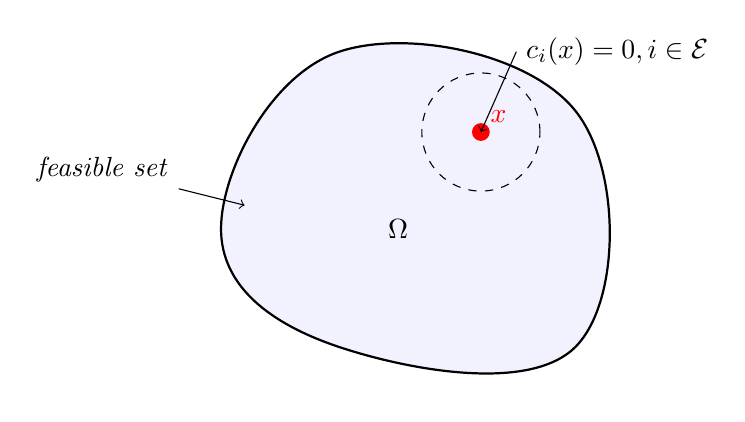
\begin{tikzpicture}[scale=1.5]
    \draw[thick, fill=blue!5] plot [smooth cycle, tension=0.7] coordinates {(-1,0) (0,1.5) (2,1) (2,-1) (0,-1)};
    \node at (0.5, 0) {$\Omega$};
    
    \node (feasible) at (-2, 0.5) {\textit{feasible set}};
    \draw[->] (feasible) -- (-0.8, 0.2);
    
    \coordinate (x) at (1.2, 0.82); % Approximate boundary point
    \filldraw[red] (x) circle (2pt) node[above right] {$x$};
    
    \draw[dashed] (x) circle (0.5cm);
    
    \draw[->] (1.5, 1.5) node[right] {$c_i(x)=0, i \in \mathcal{E}$} -- (x);
    
\end{tikzpicture}
\caption{Illustration of the feasible set $\Omega$ and a point $x$ on the boundary where some constraints are active.}
\label{fig:active-set}
\end{figure}

\begin{figureexplanation}
\textbf{Geometric interpretation:}
\begin{itemize}
    \item The set $\Omega$ is the feasible region (in blue).
    \item The point $x$ is on the boundary. Constrains are active ($c_i(x)=0$) if the boundary passes exactly through $x$.
    \item The other constraints (inactive) satisfy $c_i(x) > 0$ and do not \emph{locally} limit infinitesimal movements around $x$.
\end{itemize}
\end{figureexplanation}

\section{Examples}

\subsection{One Equality Constraint}

Consider the following minimization problem in $\mathbb{R}^2$:
\begin{equation}
    \min_{(x_1, x_2) \in \mathbb{R}^2} x_1 + x_2 \quad \text{subject to} \quad x_1^2 + x_2^2 - 2 = 0.
\end{equation}
We have:
\begin{align*}
    f(x) &= x_1 + x_2, \\
    c_1(x) &= x_1^2 + x_2^2 - 2, \\
    \mathcal{E} &= \{1\}, \quad \mathcal{I} = \emptyset.
\end{align*}
The feasible set is the circle centered at $(0,0)$ with radius $\sqrt{2}$.
Let's compute the gradients:
\begin{equation}
    \nabla f(x) = \begin{pmatrix} 1 \\ 1 \end{pmatrix}, \quad \nabla c_1(x) = \begin{pmatrix} 2x_1 \\ 2x_2 \end{pmatrix}.
\end{equation}

Note that $\nabla f(x)$ is constant (the same at every point), unlike $\nabla c_1(x)$ which depends on the position on the circle.

\begin{figure}[H]
\centering
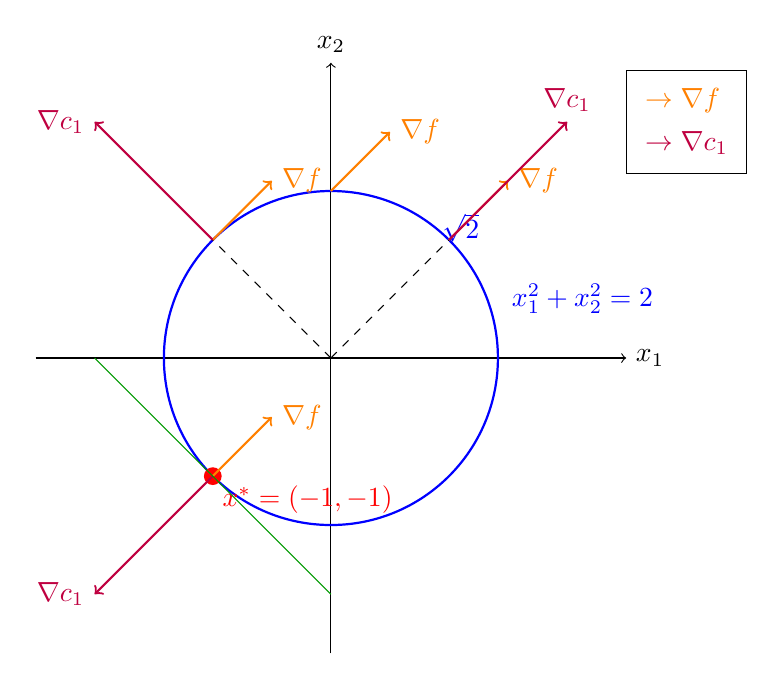
\begin{tikzpicture}[scale=1.5]
    \draw[->] (-2.5,0) -- (2.5,0) node[right] {$x_1$};
    \draw[->] (0,-2.5) -- (0,2.5) node[above] {$x_2$};
    
    \draw[thick, blue] (0,0) circle (1.414);
    \node[blue] at (1.1, 1.1) {$\sqrt{2}$};
    \node[blue, right] at (1.45, 0.5) {$x_1^2+x_2^2=2$};
    
    
    \coordinate (P1) at (1,1);
    \draw[dashed] (0,0) -- (P1);
    % grad f = (1,1) -> visual (0.5, 0.5)
    \draw[->, orange, thick] (P1) -- ++(0.5, 0.5) node[right] {$\nabla f$};
    % grad c1 = (2,2) -> visual (1, 1) -> 2x larger
    \draw[->, purple, thick] (P1) -- ++(1.0, 1.0) node[above] {$\nabla c_1$};
    
    \coordinate (P2) at (-1,1);
    \draw[dashed] (0,0) -- (P2);
    % grad f = (1,1) -> visual (0.5, 0.5)
    \draw[->, orange, thick] (P2) -- ++(0.5, 0.5) node[right] {$\nabla f$}; 
    % grad c1 = (-2,2) -> visual (-1, 1) -> 2x larger
    \draw[->, purple, thick] (P2) -- ++(-1.0, 1.0) node[left] {$\nabla c_1$};
    
    \coordinate (Opt) at (-1,-1);
    \filldraw[red] (Opt) circle (2pt);
    \node[red, below right] at (-1, -1) {$x^* = (-1, -1)$};
    
    % grad f = (1,1) -> visual (0.5, 0.5)
    \draw[->, orange, thick] (Opt) -- ++(0.5, 0.5) node[right] {$\nabla f$};
    % grad c1 = (-2,-2) -> visual (-1, -1) -> 2x larger
    \draw[->, purple, thick] (Opt) -- ++(-1.0, -1.0) node[left] {$\nabla c_1$};
    
    % Tangent line at Opt (x+y = -2)
    \draw[green!60!black, thin] (-2, 0) -- (0, -2);
    
    % Another point to show "reducing function" idea
    % Intermediate point on circle, e.g., (0, sqrt(2)) ~ (0, 1.414)
    \coordinate (P3) at (0, 1.414);
    % grad f = (1,1) -> visual (0.5, 0.5)
    \draw[->, orange, thick] (P3) -- ++(0.5, 0.5) node[right] {$\nabla f$};
    % grad c1 = (0, 2*sqrt(2)) -> direction (0,1)
    % Just showing f here to unclutter
    
    \matrix [draw, fill=white, right] at (2.5, 2) {
      \node[orange] {$\to \nabla f$}; \\
      \node[purple] {$\to \nabla c_1$}; \\
    };
\end{tikzpicture}
\caption{Minimization of $x_1+x_2$ on the circle. At the optimal point $x^*=(-1,-1)$, the gradients $\nabla f$ and $\nabla c_1$ are collinear and pointing in opposite directions. Note that $\|\nabla c_1(x)\| = 2\|\nabla f(x)\|$ on the circle.}
\label{fig:ex-equality-constraint}
\end{figure}

\begin{figureexplanation}
\textbf{Comments:}
\begin{itemize}
    \item \textbf{Variation of the objective function}: From any point on the circle (other than the optimum), it is possible to move along the circle ("reduce the function while staying on the circle") to decrease the value of $f$.
    \item \textbf{Behavior of the gradients}: The gradient of the objective function $\nabla f$ is the same at every point (constant vector $(1,1)$), unlike the constraint vectors $\nabla c_1(x)$ which change direction depending on the point considered on the circle (radial vectors).
    \item \textbf{Optimality condition}: At the optimum $x^*=(-1,-1)$, it is no longer possible to decrease $f$ while remaining on the circle. Geometrically, this corresponds to the point where the level curves of $f$ are tangent to the circle. Algebraically, we observe that $\nabla f(x^*)$ and $\nabla c_1(x^*)$ are collinear.
\end{itemize}
\end{figureexplanation}

\begin{remarque}
At the point $x^* = (-1, -1)$, the gradient of the constraint $\nabla c_1(x^*) = \begin{pmatrix} -2 \\ -2 \end{pmatrix}$ is parallel to the gradient of the objective function $\nabla f(x^*) = \begin{pmatrix} 1 \\ 1 \end{pmatrix}$.

There exists a scalar $\lambda_1^* \in \mathbb{R}$ such that:
\begin{equation}
    \nabla f(x^*) = \lambda_1^* \nabla c_1(x^*).
\end{equation}
In this example, we find $\lambda_1^* = -1/2$.
\end{remarque}

\paragraph{Derivation (Heuristic justification)}
Let $x$ be a feasible point. A small step $s$ starting from $x$ remains feasible if, to first order:
\begin{equation}
    0 = c_1(x+s) \approx \underbrace{c_1(x)}_{=0} + \nabla c_1(x)^\top s.
\end{equation}
Therefore, to stay on the constraint surface (to first order), the step $s$ must be orthogonal to the gradient of the constraint: $\nabla c_1(x)^\top s = 0$.

Moreover, the step $s$ produces a decrease in the objective function $f$ if:
\begin{equation}
    0 > f(x+s) - f(x) \approx \nabla f(x)^\top s \quad \text{(to first order)}.
\end{equation}
That is, $\nabla f(x)^\top s < 0$ (for a sufficiently small step $s$).

If $x^*$ is a local minimum, there must be no direction $s$ that is both feasible (tangent to the constraint) and a descent direction. This implies that the gradient $\nabla f(x^*)$ must be aligned with $\nabla c_1(x^*)$. If $\nabla f(x^*)$ had a non-zero component in the tangent space, we could find an $s$ reducing $f$.

This suggests that we are looking for a direction $d$ (for example with $\|d\|=1$) such that:
\begin{equation}
    \begin{cases}
    \nabla c_1(x)^\top d = 0 \quad \text{(tangent to the surface)} \\
    \nabla f(x)^\top d < 0 \quad \text{(descent)}
    \end{cases}
\end{equation}
If there is no such $d$, then it is likely that $x$ is a local minimizer.

This can only be the case if $\nabla f(x)$ and $\nabla c_1(x)$ are parallel, i.e.:
\begin{equation}
    \nabla f(x) = \lambda_1 \nabla c_1(x) \quad \text{for some } \lambda_1 \in \mathbb{R}.
\end{equation}

Otherwise, we can explicitly construct a \textit{projected} descent direction using the following formula:
\begin{equation}
    \bar{d} = - \left( I - \frac{\nabla c_1(x) \nabla c_1(x)^\top}{\|\nabla c_1(x)\|^2} \right) \nabla f(x).
\end{equation}
By normalizing $d = \frac{\bar{d}}{\|\bar{d}\|}$ (if $\bar{d} \neq 0$), this direction satisfies $\nabla c_1(x)^\top d = 0$ and $\nabla f(x)^\top d < 0$.

\begin{remarque}[Orthogonal projector]
The matrix $P = I - \frac{\nabla c_1(x) \nabla c_1(x)^\top}{\|\nabla c_1(x)\|^2}$ is the \textbf{orthogonal projector} onto the null space of $\nabla c_1(x)^\top$, i.e., onto the tangent space to the constraint surface at $x$. Thus, $\bar{d}$ is the projection of $-\nabla f(x)$ (steepest descent direction) onto this tangent space.
\end{remarque}

\begin{figure}[H]
\centering
\begin{subfigure}[b]{0.45\textwidth}
    \centering
    \begin{tikzpicture}[scale=1.2]
        \draw[thick] (0,-1.5) -- (0,1.5);
        \fill[pattern=north east lines, pattern color=gray!30] (-1.5,-1.5) rectangle (0,1.5);
        
        \coordinate (x) at (0,0);
        \filldraw (x) circle (1.5pt) node[below right] {$x$};
        
        \draw[->, purple, thick] (x) -- (1,0) node[right] {$\nabla c_1$};
        \draw[->, orange, thick] (x) -- (1,1) node[right] {$\nabla f$};
        
        % Projected direction d (tangent, down)
        % Projection of (1,1) onto line x=0 is (0,1). 
        % d should be opposite to projection -> (0,-1)
        \draw[->, green!60!black, very thick] (x) -- (0,-1) node[right] {$\bar{d}$};
        
        \node[below, align=center] at (0,-1.7) {Non-parallel case: \\ $\bar{d} \neq 0$ (descent possible)};
    \end{tikzpicture}
\end{subfigure}
\hfill
\begin{subfigure}[b]{0.45\textwidth}
    \centering
    \begin{tikzpicture}[scale=1.2]
        \draw[thick] (0,-1.5) -- (0,1.5);
        \fill[pattern=north east lines, pattern color=gray!30] (-1.5,-1.5) rectangle (0,1.5);
        
        \coordinate (x) at (0,0);
        \filldraw (x) circle (1.5pt) node[below right] {$x$};
        
        \draw[->, purple, thick] (x) -- (1.5,0) node[right] {$\nabla c_1$};
        \draw[->, orange, thick] (x) -- (0.75,0) node[above] {$\nabla f$};
        
        % No descent direction tangent
        \node[red, align=center] at (1, -1) {No tangent \\ descent direction};
        
        \node[below, align=center] at (0,-1.7) {Parallel case: \\ $\nabla f \parallel \nabla c_1 \implies \bar{d}=0$};
    \end{tikzpicture}
\end{subfigure}
\caption{Comparison of cases: On the left, $\nabla f$ is not collinear to $\nabla c_1$, the projection $\bar{d}$ provides a tangent descent direction. On the right, the gradients are collinear, no tangent descent is possible (optimality condition).}
\label{fig:projection-cases}
\end{figure}

\begin{figureexplanation}
\textbf{Interpretation:} The projected direction $\bar{d}$ only exists if $\nabla f$ and $\nabla c_1$ are not collinear. When they are parallel, any tangent component of $-\nabla f$ is zero: we cannot descend while staying on the constraint.
\end{figureexplanation}

\begin{figure}[H]
\centering
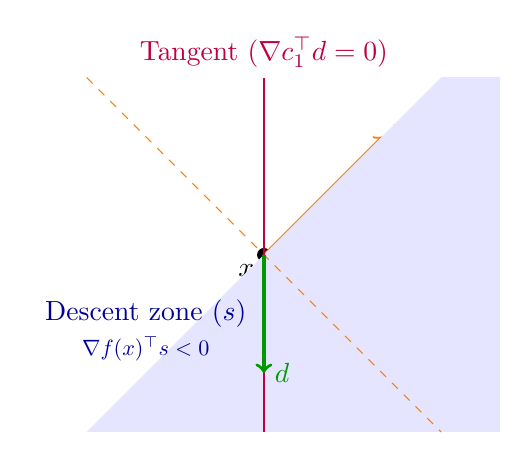
\begin{tikzpicture}[scale=1.5]
    \coordinate (x) at (0,0);
    \filldraw (x) circle (1.5pt) node[below left] {$x$};
    
    \draw[->, orange, thick] (x) -- (1, 1) node[right] {$\nabla f(x)$};
    \draw[->, purple, thick] (x) -- (1, 0) node[right] {$\nabla c_1(x)$};
    
    % Descent zone (Blue zone) - Half plane defined by grad f . d < 0
    % Normal to grad f is (-1, 1). Line passing through origin.
    \begin{scope}
        \clip (-2, -1.5) rectangle (2, 1.5);
        % Rotate coordinate system so x-axis aligns with grad f? No, simpler.
        % Just fill a large rectangle rotated.
        \fill[blue!10, rotate=-135] (-3, 0) rectangle (3, 3);
    \end{scope}
    
    \draw[dashed, orange] (-1.5, 1.5) -- (1.5, -1.5);
    \node[blue!60!black] at (-1, -0.5) {Descent zone ($s$)};
    \node[blue!60!black, scale=0.8] at (-1, -0.8) {$\nabla f(x)^\top s < 0$};
    
    \draw[thick, purple] (0, -1.5) -- (0, 1.5) node[above] {Tangent ($\nabla c_1^\top d = 0$)};
    
    % In this specific drawing, the tangent line DOES intersect the blue zone (at the bottom)
    % grad f is at 45 deg, Blue zone is roughly 135 to 315 deg.
    % grad c1 is at 0 deg. Tangent is 90/-90 deg.
    % 90 deg is NOT in blue zone (prod with (1,1) is > 0)
    % -90 deg IS in blue zone (prod with (1,1) is < 0)
    % So there IS a descent direction here!
    
    \draw[->, green!60!black, very thick] (0, 0) -- (0, -1) node[right] {$d$};
    
\end{tikzpicture}
\caption{Illustration of the direction search. The blue zone represents the set of descent directions (forming an obtuse angle with $\nabla f$). The vertical line represents the directions tangent to the constraint. Here, a direction $d$ exists (intersection of the line and the blue zone), so $x$ is not an optimum.}
\label{fig:direction-finding}
\end{figure}

\begin{figureexplanation}
\textbf{Interpretation:} We look for a direction $d$ such that $\nabla f^\top d < 0$ (descent) and $\nabla c_1^\top d = 0$ (tangent). If the tangent line passes through the blue zone, such a direction exists and $x$ is not optimal.
\end{figureexplanation}

\paragraph{Lagrangian function}
Let us define the Lagrangian function:
\begin{equation}
    \mathcal{L}(x, \lambda_1) = f(x) - \lambda_1 c_1(x).
\end{equation}
Its gradient with respect to $x$ is:
\begin{equation}
    \nabla_x \mathcal{L}(x, \lambda_1) = \nabla f(x) - \lambda_1 \nabla c_1(x).
\end{equation}
The condition for the gradients to be parallel can then be rewritten as follows:
\begin{quote}
There exists $\lambda_1^* \in \mathbb{R}$ such that $\nabla_x \mathcal{L}(x^*, \lambda_1^*) = 0$.
\end{quote}
This suggests that we must look for the stationary points of $\mathcal{L}$ to find the constrained minimizers of $f$.

\begin{remarque}
The point $(1, 1)$ is also a stationary point of $\mathcal{L}$ (with a different Lagrange multiplier). It corresponds here to the global maximum of $f$ on the circle.
\end{remarque}

\subsection{One Inequality Constraint}

Now consider the problem with one inequality constraint:
\begin{equation}
    \min_{(x_1, x_2) \in \mathbb{R}^2} x_1 + x_2 \quad \text{subject to} \quad 2 - x_1^2 - x_2^2 \geq 0.
\end{equation}
The constraint is $c_1(x) = 2 - x_1^2 - x_2^2 \geq 0$. The feasible set is the closed disk of radius $\sqrt{2}$. The solution is still the same point $x^* = (-1, -1)$.

Let's compute the gradients at $x^*$:
\begin{align*}
    \nabla f(x^*) &= \begin{pmatrix} 1 \\ 1 \end{pmatrix}, \\
    \nabla c_1(x) &= \begin{pmatrix} -2x_1 \\ -2x_2 \end{pmatrix} \implies \nabla c_1(x^*) = \begin{pmatrix} 2 \\ 2 \end{pmatrix}.
\end{align*}

The parallelism condition:
\begin{equation}
    \nabla f(x^*) = \lambda_1^* \nabla c_1(x^*)
\end{equation}
is satisfied for $\lambda_1^* = \frac{1}{2}$. Note that this time, $\lambda_1^* > 0$.

\begin{remarque}[Interpretation of the positive multiplier]
The fact that $\lambda_1^* > 0$ indicates that the constraint is \textbf{binding}: relaxing this constraint would allow $f$ to be decreased further. Indeed, if one could "go outside" the disk (i.e.\ move in the direction $-\nabla f$), one could continue to decrease the objective function. The multiplier $\lambda^*$ quantifies this "pressure" of the constraint at the optimum.
\end{remarque}

\begin{figure}[H]
\centering
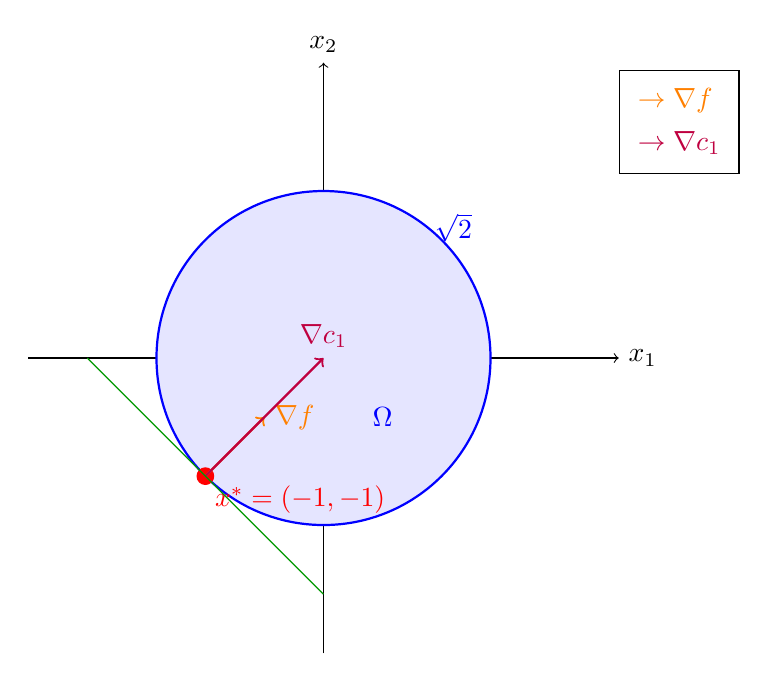
\begin{tikzpicture}[scale=1.5]
    \draw[->] (-2.5,0) -- (2.5,0) node[right] {$x_1$};
    \draw[->] (0,-2.5) -- (0,2.5) node[above] {$x_2$};
    
    \filldraw[fill=blue!10, draw=blue, thick] (0,0) circle (1.414);
    \node[blue] at (0.5, -0.5) {$\Omega$};
    \node[blue] at (1.1, 1.1) {$\sqrt{2}$};
    
    \coordinate (Opt) at (-1,-1);
    \filldraw[red] (Opt) circle (2pt);
    \node[red, below right] at (-1, -1) {$x^* = (-1, -1)$};
    
    % grad f is (1,1) -> visual (0.5, 0.5) points "inward" (towards origin)
    \draw[->, orange, thick] (Opt) -- ++(0.5, 0.5) node[right] {$\nabla f$};
    
    % grad c1 is (2,2) -> visual (1, 1) points "inward" (same direction)
    \draw[->, purple, thick] (Opt) -- ++(1.0, 1.0) node[above] {$\nabla c_1$};
    
    % Tangent line
    \draw[green!60!black, thin] (-2, 0) -- (0, -2);
    
    \matrix [draw, fill=white, right] at (2.5, 2) {
      \node[orange] {$\to \nabla f$}; \\
      \node[purple] {$\to \nabla c_1$}; \\
    };
\end{tikzpicture}
\caption{Minimization with an inequality constraint. At the optimal point, $\nabla f$ and $\nabla c_1$ point in the same direction ($\lambda^* > 0$).}
\label{fig:ex-inequality-constraint}
\end{figure}

\begin{figureexplanation}
\textbf{Interpretation:} Unlike the equality case, the gradients point in the \textbf{same direction}. The multiplier $\lambda^* > 0$ reflects the fact that the constraint "pushes" the optimum: without it, we could descend further.
\end{figureexplanation}

\paragraph{Derivation (Heuristic justification)}
Let $x$ be a feasible point.
A small step $s$ starting from $x$ produces a decrease in the objective function if, to first order:
\begin{equation}
    \nabla f(x)^\top s < 0.
\end{equation}
This step preserves feasibility with respect to the constraint $c_1$ if:
\begin{equation}
    0 \le c_1(x+s) \approx c_1(x) + \nabla c_1(x)^\top s.
\end{equation}
Thus, to first order, we must have:
\begin{equation}
    c_1(x) + \nabla c_1(x)^\top s \ge 0.
\end{equation}

We then distinguish two cases:
\begin{enumerate}
    \item \textbf{$x$ is strictly inside the domain} (i.e. $c_1(x) > 0$). \\
    Any sufficiently small step $s$ will ensure that $c_1(x) + \nabla c_1(x)^\top s \ge 0$. For instance, one can choose the direction of steepest descent $s = -\alpha \nabla f(x)$ with $\alpha > 0$ small (if $\nabla f(x) \neq 0$). In this case, the constraint is not \textit{active} and does not locally limit the minimization.
    
    \item \textbf{$x$ is on the boundary of the feasible set} (i.e. $c_1(x) = 0$). \\
    In this case, the conditions for function decrease and feasibility become:
    \begin{equation}
        \nabla f(x)^\top s < 0 \quad \text{and} \quad \nabla c_1(x)^\top s \ge 0.
    \end{equation}
    At the optimum, there must be no such $s$. This implies a specific relationship between the gradients (see KKT condition later).
\end{enumerate}



\begin{figure}[H]
\centering
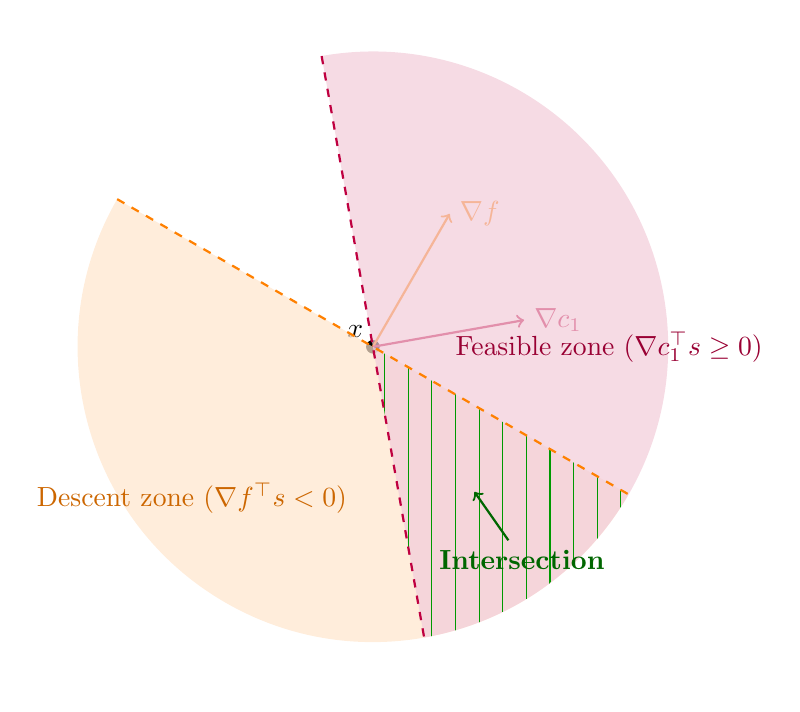
\begin{tikzpicture}[scale=1.5]
    \coordinate (x) at (0,0);
    \filldraw (x) circle (1.5pt) node[above left] {$x$};
    
    % Vectors setup
    % grad f at 60 degrees
    \draw[->, orange, thick] (x) -- (60:1.3) node[right] {$\nabla f$};
    % grad c1 moved to 10 degrees (closer to grad f to tighten intersection)
    \draw[->, purple, thick] (x) -- (10:1.3) node[right] {$\nabla c_1$};
    
    % Half-Plane 1: Descent (Orange)
    % Perpendicular to grad f (150 to 330).
    \begin{scope}
        \fill[orange!20, opacity=0.7] (0,0) -- (150:2.5) arc (150:330:2.5) -- cycle;
    \end{scope}
     \node[orange!80!black] at (220:2.0) {Descent zone ($\nabla f^\top s < 0$)};

    % Perpendicular to grad c1 (normal at 10 deg -> boundary at 100/280).
    % Valid region is same side as grad c1 -> Angles [-80, 100] i.e. [280, 460].
    \begin{scope}
        \fill[purple!20, opacity=0.7] (0,0) -- (100:2.5) arc (100:-80:2.5) -- cycle;
    \end{scope}
    \node[purple!80!black] at (0:2.0) {Feasible zone ($\nabla c_1^\top s \geq 0$)};

    % Width = 50 degrees (tighter than 90).
    \begin{scope}
        \clip (0,0) -- (280:2.5) arc (280:330:2.5) -- cycle;
        \foreach \x in {-2.5,-2.3,...,2.5} \draw[green!60!black, thin] (\x,-2.5) -- (\x,2.5);
    \end{scope}
    
    % Boundaries lines
    \draw[dashed, orange, thick] (150:2.5) -- (330:2.5);
    \draw[dashed, purple, thick] (100:2.5) -- (280:2.5); % Boundary for grad c1 at 10 deg

    \node[green!40!black, font=\bfseries] at (305:2.2) {Intersection};
    \draw[->, green!40!black, thick] (305:2.0) -- (305:1.5);
    
\end{tikzpicture}
\caption{Visualization of acceptable directions. The two colored zones (orange for descent, purple for feasibility) overlap. The intersection (hatched in green) represents the set of acceptable directions.}
\label{fig:acceptable-directions-overlap}
\end{figure}

\begin{figureexplanation}
\textbf{Geometric interpretation:}
\begin{itemize}
    \item For a direction $s$ to be a \textbf{descent direction}, it must form an obtuse angle with the gradient of the objective function $\nabla f$ (orange zone).
    \item For it to be \textbf{feasible} (to first order), it must point towards the interior of the domain with respect to the active constraint, hence forming an acute angle with the gradient of the constraint $\nabla c_1$ (purple zone).
    \item The \textbf{intersection} (green hatching) contains the acceptable directions. As long as this intersection is not empty, the solution can be improved.
\end{itemize}
\end{figureexplanation}

The fundamental question then becomes: \textbf{When is there no acceptable direction?}

\begin{figure}[H]
\centering
\begin{subfigure}[b]{0.45\textwidth}
    \centering
    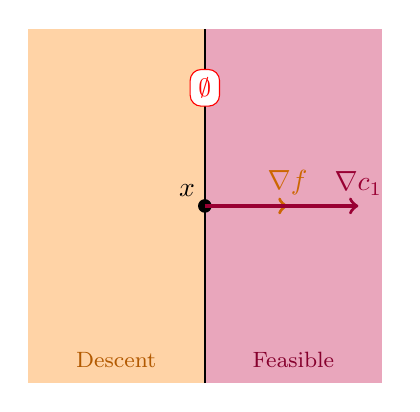
\begin{tikzpicture}[scale=1.5]
        % CASE 1: No acceptable direction - CLEAN VERSION
        \coordinate (x) at (0,0);
        
        % Zone de descente (left, orange transparent)
        \fill[orange, opacity=0.35] (-1.5,-1.5) rectangle (0,1.5);
        
        % Zone réalisable (right, purple transparent)
        \fill[purple, opacity=0.35] (0,-1.5) rectangle (1.5,1.5);
        
        % Boundary line
        \draw[thick, black] (0,-1.5) -- (0,1.5);
        
        \filldraw (x) circle (1.5pt) node[above left] {$x$};
        
        \draw[->, orange!80!black, very thick] (x) -- (0.7, 0) node[above] {$\nabla f$};
        \draw[->, purple!80!black, very thick] (x) -- (1.3, 0) node[above] {$\nabla c_1$};
        
        \node[orange!70!black, font=\footnotesize] at (-0.75, -1.3) {Descent};
        \node[purple!70!black, font=\footnotesize] at (0.75, -1.3) {Feasible};
        
        \node[red, font=\small\bfseries, fill=white, draw=red, inner sep=3pt, rounded corners] at (0, 1.0) {$\emptyset$};
        
    \end{tikzpicture}
    \caption{Aligned gradients: disjoint zones, no acceptable direction.}
\end{subfigure}
\hfill
\begin{subfigure}[b]{0.45\textwidth}
    \centering
    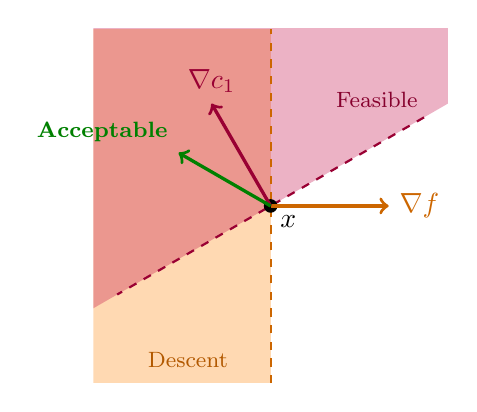
\begin{tikzpicture}[scale=1.5]
        % CASE 2: Overlapping transparent zones
        \coordinate (x) at (0,0);
        
        \begin{scope}
            \clip (-1.5,-1.5) rectangle (1.5,1.5);
            
            % Zone de descente (orange, transparent)
            \fill[orange, opacity=0.3] (-1.5,-1.5) rectangle (0,1.5);
            
            % Zone réalisable (purple, transparent) - overlaps naturally
            \fill[purple, opacity=0.3] (0,0) -- (30:3) arc (30:210:3) -- cycle;
        \end{scope}
        
        % Boundaries
        \draw[dashed, orange!80!black, thick] (0, -1.5) -- (0, 1.5);
        \draw[dashed, purple!80!black, thick] (30:1.5) -- (210:1.5);
        
        \filldraw (x) circle (1.5pt) node[below right] {$x$};
        
        \draw[->, orange!80!black, very thick] (x) -- (1, 0) node[right] {$\nabla f$};
        \draw[->, purple!80!black, very thick] (x) -- (120:1.0) node[above] {$\nabla c_1$};
        
        \node[orange!70!black, font=\footnotesize] at (-0.7, -1.3) {Descent};
        \node[purple!70!black, font=\footnotesize] at (0.9, 0.9) {Feasible};
        
        % Arrow indicating intersection zone
        \draw[->, green!50!black, very thick] (x) -- (150:0.9) node[above left, font=\footnotesize\bfseries] {Acceptable};
        
    \end{tikzpicture}
    \caption{Regular case: The intersection of the zones (color mixing) gives the acceptable directions.}
\end{subfigure}
\caption{Comparison of "Half-plane" configurations. On the left, parallel gradients in the same direction create a total obstruction (perfect opposition of zones).}
\label{fig:admissible-comparison}
\end{figure}

\begin{figureexplanation}
\textbf{Geometric interpretation:}
\begin{itemize}
    \item \textbf{Case (a):} The descent and feasibility zones are disjoint (no overlap). This is the optimality condition.
    \item \textbf{Case (b):} The two zones overlap through color transparency. The intersection (darker) gives the acceptable directions.
\end{itemize}
\end{figureexplanation}

We deduce the following conclusion:
\begin{quote}
There is no acceptable direction when the gradients are parallel and point in the same direction:
\begin{equation}
    \nabla f(x) = \lambda \nabla c_1(x) \quad \text{with } \lambda > 0.
\end{equation}
\end{quote}

\paragraph{Summary of the two cases (Optimality conditions)}
When there is no feasible descent direction, we have the following system:
\begin{equation}
    \begin{cases}
        \nabla_x \mathcal{L}(x, \lambda_1^*) = 0 \quad \text{for some } \lambda_1^* \ge 0, \\
        \lambda_1^* c_1(x) = 0.
    \end{cases}
\end{equation}
The second equation is called the \textbf{complementarity condition}.
It means that the multiplier $\lambda_1^*$ can only be (strictly) positive if the constraint $c_1$ is active ($c_1(x)=0$).

Recall the definition of the Lagrangian:
\begin{equation}
    \mathcal{L}(x, \lambda_1) = f(x) - \lambda_1 c_1(x).
\end{equation}
If $\lambda_1 = 0$, then $\mathcal{L}(x, \lambda_1) = f(x)$ and $\nabla_x \mathcal{L} = \nabla f(x)$. This corresponds to the case where the optimum is inside the domain (inactive constraint), and we recover the classic condition $\nabla f(x) = 0$.

\subsection{Two Inequality Constraints}

Consider the following problem:
\begin{equation}
    \min_{(x_1, x_2) \in \mathbb{R}^2} x_1 + x_2 \quad \text{subject to} \quad 
    \begin{cases}
        2 - x_1^2 - x_2^2 \ge 0, \\
        x_2 \ge 0.
    \end{cases}
\end{equation}
The feasible set is the upper half of the disk of radius $\sqrt{2}$.
The optimal point is $x^* = (-\sqrt{2}, 0)$.

Let's compute the gradients at this point:
\begin{align*}
    \nabla f(x) &= \begin{pmatrix} 1 \\ 1 \end{pmatrix}, \\
    \nabla c_1(x) &= \begin{pmatrix} -2x_1 \\ -2x_2 \end{pmatrix} \implies \nabla c_1(x^*) = \begin{pmatrix} 2\sqrt{2} \\ 0 \end{pmatrix}, \\
    \nabla c_2(x) &= \begin{pmatrix} 0 \\ 1 \end{pmatrix} \implies \nabla c_2(x^*) = \begin{pmatrix} 0 \\ 1 \end{pmatrix}.
\end{align*}
Note that both constraints are active at $x^*$ ($c_1(x^*) = 0$ and $c_2(x^*) = 0$).

We would expect a feasible descent direction $d$ to satisfy:
\begin{equation}
    \begin{cases}
        \nabla c_i(x^*)^\top d \ge 0 \quad \text{for } i=1, 2 \quad \text{(feasible)}, \\
        \nabla f(x^*)^\top d < 0 \quad \text{(descent)}.
    \end{cases}
\end{equation}

\begin{figure}[H]
\centering
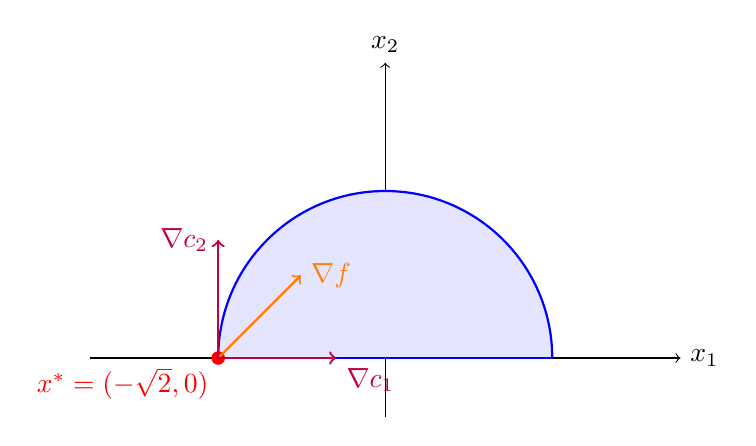
\begin{tikzpicture}[scale=1.5]
    \draw[->] (-2.5,0) -- (2.5,0) node[right] {$x_1$};
    \draw[->] (0,-0.5) -- (0,2.5) node[above] {$x_2$};
    
    \fill[blue!10] (1.414, 0) arc (0:180:1.414) -- cycle;
    \draw[blue, thick] (1.414, 0) arc (0:180:1.414);
    \draw[blue, thick] (-1.414, 0) -- (1.414, 0);
    
    \coordinate (Opt) at (-1.414, 0);
    \filldraw[red] (Opt) circle (1.5pt) node[below left] {$x^* = (-\sqrt{2}, 0)$};
    
    \draw[->, orange, thick] (Opt) -- ++(0.7, 0.7) node[right] {$\nabla f$};
    
    \draw[->, purple, thick] (Opt) -- ++(1.0, 0) node[below right] {$\nabla c_1$};
    
    \draw[->, purple, thick] (Opt) -- ++(0, 1.0) node[left] {$\nabla c_2$};
    
    % Cone of feasible directions?
    % Descent directions roughly Left-Down sector
    % No interaction.
    
\end{tikzpicture}
\caption{Example with two active constraints. Both constraints (disk and non-negativity) are active at $x^*$.}
\label{fig:ex-two-inequalities}
\end{figure}

\begin{figureexplanation}
\textbf{Situation with multiple active constraints:}
Here, the point $x^*$ is at the intersection of two boundaries ($c_1=0$ for the circle, $c_2=0$ for the horizontal line).
\begin{itemize}
    \item The gradient $\nabla f$ must be a linear combination with positive coefficients of the gradients of the active constraints ($\nabla c_1$ and $\nabla c_2$).
    \item Geometrically, this means that $-\nabla f$ (desired descent direction) points outside the cone formed by the tangents to the constraints. We are "blocked" by both walls at once.
\end{itemize}
\end{figureexplanation}

\paragraph{Modification of the Lagrangian}
For this problem with two constraints, we define the Lagrangian:
\begin{equation}
    \mathcal{L}(x, \lambda) = f(x) - \lambda_1 c_1(x) - \lambda_2 c_2(x).
\end{equation}
The conditions become:
\begin{itemize}
    \item $\nabla_x \mathcal{L}(x^*, \lambda^*) = 0$ with $\lambda^* \ge 0$ (i.e., $\lambda_1^* \ge 0$ and $\lambda_2^* \ge 0$).
    \item Complementarity conditions: $\lambda_1^* c_1(x^*) = 0$ and $\lambda_2^* c_2(x^*) = 0$.
\end{itemize}

Let's check these conditions for our point $x^* = (-\sqrt{2}, 0)$.
We look for $\lambda_1^*, \lambda_2^*$ such that:
\begin{align*}
    \nabla f(x^*) - \lambda_1^* \nabla c_1(x^*) - \lambda_2^* \nabla c_2(x^*) &= 0 \\
    \begin{pmatrix} 1 \\ 1 \end{pmatrix} - \lambda_1^* \begin{pmatrix} 2\sqrt{2} \\ 0 \end{pmatrix} - \lambda_2^* \begin{pmatrix} 0 \\ 1 \end{pmatrix} &= \begin{pmatrix} 0 \\ 0 \end{pmatrix}.
\end{align*}
This system gives:
\begin{equation}
    \begin{cases}
        1 - 2\sqrt{2} \lambda_1^* = 0 \implies \lambda_1^* = \frac{1}{2\sqrt{2}} > 0, \\
        1 - \lambda_2^* = 0 \implies \lambda_2^* = 1 > 0.
    \end{cases}
\end{equation}
The multipliers are positive, which is consistent with the fact that both constraints are active and restrict descent.
\paragraph{Analysis of another candidate point}
Consider the point $x = (\sqrt{2}, 0)$. This point is feasible (on the boundary).
Let's check if the optimality conditions are satisfied.
\begin{align*}
    \nabla f(x) &= \begin{pmatrix} 1 \\ 1 \end{pmatrix}, \\
    \nabla c_1(x) &= \begin{pmatrix} -2\sqrt{2} \\ 0 \end{pmatrix}, \\
    \nabla c_2(x) &= \begin{pmatrix} 0 \\ 1 \end{pmatrix}.
\end{align*}
We look for $\lambda_1^*, \lambda_2^*$ such that:
\begin{equation}
    \begin{pmatrix} 1 \\ 1 \end{pmatrix} - \lambda_1^* \begin{pmatrix} -2\sqrt{2} \\ 0 \end{pmatrix} - \lambda_2^* \begin{pmatrix} 0 \\ 1 \end{pmatrix} = \begin{pmatrix} 0 \\ 0 \end{pmatrix}.
\end{equation}
This gives the system:
\begin{equation}
    \begin{cases}
        1 + 2\sqrt{2} \lambda_1^* = 0 \implies \lambda_1^* = -\frac{1}{2\sqrt{2}} < 0, \\
        1 - \lambda_2^* = 0 \implies \lambda_2^* = 1 \ge 0.
    \end{cases}
\end{equation}
Here, we find $\lambda_1^* < 0$. The KKT condition $\lambda^* \ge 0$ is not met.
\textbf{Conclusion:} The point $x = (\sqrt{2}, 0)$ is not a local minimum (indeed, we could increase $x_1$ to decrease $f$ while staying in the domain).

\section{Tangent Cone and Constraint Qualifications}

In this section, we will study the conditions under which analytical and geometrical points of view coincide.

\subsection{Definitions}

\begin{definition}[Feasible Sequence]
    A sequence $(z_k)_k$ is said to be a \textbf{feasible sequence approaching the feasible point} $x$ if:
    \begin{itemize}
        \item $z_k \to x$ as $k \to \infty$,
        \item $z_k \in \Omega$ for large enough $k$.
    \end{itemize}
\end{definition}

\begin{definition}[Tangent Vector]
    A vector $d \in \mathbb{R}^n$ is said to be \textbf{tangent} (or tangent vector) to $\Omega$ at the feasible point $x$ if there exists a feasible sequence $(z_k)_k$ approaching $x$ and a sequence of positive scalars $(t_k)_k$ with $t_k \to 0$ such that:
    \begin{equation}
        \lim_{k \to \infty} \frac{z_k - x}{t_k} = d.
    \end{equation}
\end{definition}



The set of tangent vectors to $\Omega$ at $x$ is denoted $T_\Omega(x)$ and is called the \textbf{tangent cone} to $\Omega$ at $x$.

\begin{remarque}
    $T_\Omega(x)$ is indeed a cone:
    \begin{itemize}
        \item $0 \in T_\Omega(x)$ (take the constant sequence $z_k = x$).
        \item If $d \in T_\Omega(x)$, then for all $\alpha > 0$, $\alpha d \in T_\Omega(x)$. \\
        Indeed, one just replaces the sequence $(t_k)_k$ by $(t'_k)_k$ defined by $t'_k = \alpha^{-1} t_k$. As $t_k \to 0$, we also have $t'_k \to 0$, and
        \[ \lim_{k \to \infty} \frac{z_k - x}{t'_k} = \lim_{k \to \infty} \alpha \frac{z_k - x}{t_k} = \alpha d. \]
    \end{itemize}
\end{remarque}

\begin{definition}[Linearized Feasible Directions]
    Given a feasible point $x$ and the active set $\mathcal{A}(x)$, the set of \textbf{linearized feasible directions} $\mathcal{F}(x)$ is defined by:
    \begin{equation}
        \mathcal{F}(x) = \left\{ d \in \mathbb{R}^n \mid 
        \begin{aligned}
            d^\top \nabla c_i(x) &= 0 \quad \forall i \in \mathcal{E}, \\
            d^\top \nabla c_i(x) &\ge 0 \quad \forall i \in \mathcal{I} \cap \mathcal{A}(x)
        \end{aligned}
        \right\}.
    \end{equation}
\end{definition}

\begin{remarque}
    $\mathcal{F}(x)$ is also a cone.
\end{remarque}

\begin{exemple}[Tangent cone for an equality constraint]
    Consider the problem:
    \begin{equation}
        \min_{x \in \mathbb{R}^2} x_1 + x_2 \quad \text{subject to} \quad x_1^2 + x_2^2 - 2 = 0.
    \end{equation}
    Let $x = (-\sqrt{2}, 0)$.
    The \textbf{feasible sequences} $(z_k)_k$ approaching $x$ must lie on the circle.
    
    Consider the feasible sequences:
    \begin{equation}
        z_k = \left(-\sqrt{2 - \frac{1}{k^2}}, \frac{1}{k}\right) \quad \text{or} \quad z'_k = \left(-\sqrt{2 - \frac{1}{k^2}}, -\frac{1}{k}\right).
    \end{equation}
    Let's check they are on the circle: $\left(-\sqrt{2-1/k^2}\right)^2 + (\pm 1/k)^2 = 2 - 1/k^2 + 1/k^2 = 2$.
    
    With $t_k = \|z_k - x\|$, we find that the vectors $(0, 1)$ and $(0, -1)$ are tangent.
    More generally, the set of tangent vectors is the vertical line:
    \begin{equation}
        T_\Omega(x) = \{ (0, d_2) \mid d_2 \in \mathbb{R} \}.
    \end{equation}

    \begin{center}
    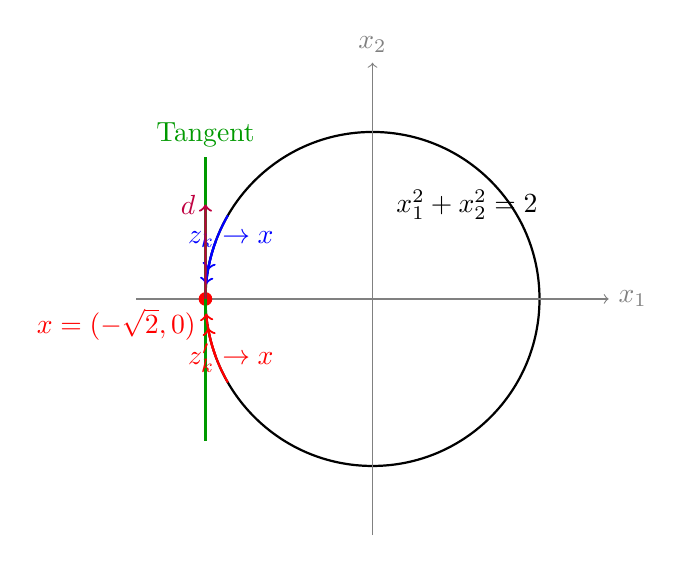
\begin{tikzpicture}[scale=1.5]
        \draw[thick] (0,0) circle (1.414);
        \node at (0.8, 0.8) {$x_1^2+x_2^2=2$};
        
        \draw[->, gray] (-2,0) -- (2,0) node[right] {$x_1$};
        \draw[->, gray] (0,-2) -- (0,2) node[above] {$x_2$};
        
        \coordinate (x) at (-1.414, 0);
        \filldraw[red] (x) circle (1.5pt) node[below left] {$x = (-\sqrt{2}, 0)$};
        
        % Tangent line (vertical)
        \draw[green!60!black, thick] (-1.414, -1.2) -- (-1.414, 1.2) node[above] {Tangent};
        
        % From top (z_k): Blue arrows approaching 180 deg from 150 deg
        \draw[->, blue, thick] (150:1.414) arc (150:170:1.414);
        \draw[->, blue, thick] (160:1.414) arc (160:175:1.414);
        \node[blue] at (-1.2, 0.5) {$z_k \to x$};

        % From bottom (z'_k): Red arrows approaching 180 deg from 210 deg
        \draw[->, red, thick] (210:1.414) arc (210:190:1.414);
        \draw[->, red, thick] (200:1.414) arc (200:185:1.414);
        \node[red] at (-1.2, -0.5) {$z'_k \to x$};
        
        % Vector d (tangent vector)
        \draw[->, purple, thick] (x) -- (-1.414, 0.8) node[left] {$d$};

    \end{tikzpicture}
    \end{center}
\end{exemple}

Now let's compute $\mathcal{F}(x)$ at $x = (-\sqrt{2}, 0)$.
    We have $\mathcal{E} = \{1\}$ and $\mathcal{I} = \emptyset$, so $\mathcal{A}(x) = \{1\}$. 
    The constraint $c_1(x) = x_1^2 + x_2^2 - 2$ has the gradient:
    \begin{equation}
        \nabla c_1(x) = \begin{pmatrix} 2x_1 \\ 2x_2 \end{pmatrix} \implies \nabla c_1(x) = \begin{pmatrix} -2\sqrt{2} \\ 0 \end{pmatrix}.
    \end{equation}
    The set of linearized feasible directions is:
    \begin{equation}
        \mathcal{F}(x) = \left\{ d = \begin{pmatrix} d_1 \\ d_2 \end{pmatrix} \in \mathbb{R}^2 \mid d^\top \nabla c_1(x) = 0 \right\}.
    \end{equation}
    The condition $d^\top \nabla c_1(x) = 0$ gives:
    \begin{equation}
        \begin{pmatrix} d_1 \\ d_2 \end{pmatrix}^\top \begin{pmatrix} -2\sqrt{2} \\ 0 \end{pmatrix} = -2\sqrt{2} d_1 = 0 \implies d_1 = 0.
    \end{equation}
    So:
    \begin{equation}
        \mathcal{F}(x) = \left\{ (0, d_2)^\top \mid d_2 \in \mathbb{R} \right\} = T_\Omega(x).
    \end{equation}

\begin{remarque}[Cases where $\mathcal{F}(x) \neq T_\Omega(x)$]
    \begin{itemize}
        \item If we change the constraint to $(x_1^2 + x_2^2 - 2)^2 = 0$, it can be shown that $\mathcal{F}(x) = \mathbb{R}^2 \neq T_\Omega(x)$.
        
        Indeed, the gradient of this new constraint at $x$ vanishes:
        \[ \nabla \left[ (x_1^2 + x_2^2 - 2)^2 \right] = 2(x_1^2 + x_2^2 - 2) \cdot \begin{pmatrix} 2x_1 \\ 2x_2 \end{pmatrix} = 0 \text{ on the circle.} \]
        Thus the condition $d^\top \nabla c(x) = 0$ is always satisfied, hence $\mathcal{F}(x) = \mathbb{R}^2$.
        
        \item If we change the constraint to $2 - x_1^2 - x_2^2 \geq 0$ (inequality), then:
        \begin{equation}
            T_\Omega(x) = \left\{ (d_1, d_2)^\top \in \mathbb{R}^2 \mid d_1 \geq 0 \right\} = \mathcal{F}(x).
        \end{equation}
    \end{itemize}
\end{remarque}

\subsection{Linear Independence Constraint Qualification (LICQ)}

\begin{definition}[LICQ -- Linear Independence Constraint Qualification]
    Given a feasible point $x \in \Omega$ and the active set $\mathcal{A}(x)$, we say that the \textbf{LICQ} condition is satisfied at $x$ if the set of gradients of the active constraints
    \begin{equation}
        \left\{ \nabla c_i(x) \mid i \in \mathcal{A}(x) \right\}
    \end{equation}
    is \textbf{linearly independent}.
\end{definition}

\begin{proposition}
    Under the LICQ condition, the tangent cone $T_\Omega(x)$ and the set of linearized feasible directions $\mathcal{F}(x)$ coincide:
    \begin{equation}
        T_\Omega(x) = \mathcal{F}(x).
    \end{equation}
\end{proposition}

\begin{lemme}[Case of linear constraints]
    Suppose that at a point $x^* \in \Omega$, all active constraints $c_i$ (for $i \in \mathcal{A}(x^*)$) are \textbf{linear} (or affine) functions. Then:
    \begin{equation}
        T_\Omega(x^*) = \mathcal{F}(x^*).
    \end{equation}
\end{lemme}

\begin{remarque}
    This lemma is a special case of the previous proposition. Linear constraints automatically satisfy LICQ if their gradients are linearly independent. Moreover, for affine constraints, the linear approximation is exact, which explains the equality $T_\Omega = \mathcal{F}$.
\end{remarque}

\section{Optimality Conditions}

In this section, we formalize the optimality conditions for constrained optimization problems. For detailed proofs, we refer to Nocedal and Wright \cite{nocedal2006numerical}.

\subsection{The Lagrangian Function}

\begin{definition}[Lagrangian Function]
    For the optimization problem
    \begin{equation}
        \min_{x \in \mathbb{R}^n} f(x) \quad \text{subject to} \quad c_i(x) \begin{cases} = 0 & \text{if } i \in \mathcal{E}, \\ \geq 0 & \text{if } i \in \mathcal{I}, \end{cases}
    \end{equation}
    the \textbf{Lagrangian function} is defined by:
    \begin{equation}
        \mathcal{L}(x, \lambda) = f(x) - \sum_{i \in \mathcal{E} \cup \mathcal{I}} \lambda_i c_i(x),
    \end{equation}
    where $\lambda = (\lambda_i)_{i \in \mathcal{E} \cup \mathcal{I}}$ is the vector of \textbf{Lagrange multipliers}.
\end{definition}

\begin{remarque}
    The sign convention can vary among authors. Our choice (minus sign before the $\lambda_i$) implies that for inequality constraints, the optimal multipliers will be positive $\lambda_i^* \geq 0$, which corresponds to the standard economic interpretation.
\end{remarque}

\subsection{KKT Conditions}

\begin{theoreme}[Karush-Kuhn-Tucker (KKT) Conditions]
    Let $x^*$ be a local minimum of the optimization problem. If LICQ is satisfied at $x^*$, then there exists a multiplier vector $\lambda^* = (\lambda_i^*)_{i \in \mathcal{E} \cup \mathcal{I}}$ such that:
    \begin{enumerate}
        \item \textbf{Stationarity:} 
        \begin{equation}
            \nabla_x \mathcal{L}(x^*, \lambda^*) = \nabla f(x^*) - \sum_{i \in \mathcal{E} \cup \mathcal{I}} \lambda_i^* \nabla c_i(x^*) = 0.
        \end{equation}
        
        \item \textbf{Primal Feasibility:}
        \begin{equation}
            c_i(x^*) = 0 \quad \forall i \in \mathcal{E}, \qquad c_i(x^*) \geq 0 \quad \forall i \in \mathcal{I}.
        \end{equation}
        
        \item \textbf{Dual Feasibility:}
        \begin{equation}
            \lambda_i^* \geq 0 \quad \forall i \in \mathcal{I}.
        \end{equation}
        (No sign constraint for $\lambda_i^*$ with $i \in \mathcal{E}$.)
        
        \item \textbf{Complementarity:}
        \begin{equation}
            \lambda_i^* c_i(x^*) = 0 \quad \forall i \in \mathcal{I}.
        \end{equation}
    \end{enumerate}
\end{theoreme}

\begin{remarque}[Interpretation of Complementarity]
    The complementarity condition $\lambda_i^* c_i(x^*) = 0$ means that:
    \begin{itemize}
        \item If an inequality constraint $i \in \mathcal{I}$ is not active ($c_i(x^*) > 0$), then the corresponding multiplier must be zero ($\lambda_i^* = 0$).
        \item A strictly positive multiplier ($\lambda_i^* > 0$) can only appear if the constraint is active ($c_i(x^*) = 0$).
    \end{itemize}
    Intuitively, only "tight" constraints exert a "force" on the optimum.
\end{remarque}

\subsection{Second-Order Conditions}

\paragraph{Assumption.} In this section III.2, we assume that $f$ and $c_i$ are \textbf{twice continuously differentiable}.

\begin{definition}[Critical Cone]
    Given $\mathcal{A}(x^*)$ and Lagrange multipliers $\lambda^*$ satisfying the KKT conditions, the \textbf{critical cone} $\mathcal{C}(x^*, \lambda^*)$ is defined by:
    \begin{equation}
        \mathcal{C}(x^*, \lambda^*) = \left\{ w \in \mathcal{F}(x^*) \mid \nabla c_i(x^*)^\top w = 0 \ \text{for all } i \in \mathcal{I} \cap \mathcal{A}(x^*) \ \text{with } \lambda_i^* > 0 \right\}.
    \end{equation}
\end{definition}

\begin{remarque}
    The critical cone is a subset of the set of linearized feasible directions $\mathcal{F}(x^*)$. It contains the "critical" directions that are orthogonal to the gradients of the inequality constraints that are both active \textbf{and} have a strictly positive multiplier.
    
    Intuitively, these are the directions along which the constraint "really counts" because it exerts a non-zero force at the optimum.
\end{remarque}

\begin{remarque}[Equivalence for the critical cone]
    Equivalently, one can characterize the critical cone by:
    \begin{equation}
        w \in \mathcal{C}(x^*, \lambda^*) \iff 
        \begin{cases}
            \nabla c_i(x^*)^\top w = 0 & \text{for all } i \in \mathcal{E}, \\
            \nabla c_i(x^*)^\top w \geq 0 & \text{for all } i \in \mathcal{I} \cap \mathcal{A}(x^*) \text{ with } \lambda_i^* = 0, \\
            \nabla c_i(x^*)^\top w = 0 & \text{for all } i \in \mathcal{I} \cap \mathcal{A}(x^*) \text{ with } \lambda_i^* > 0.
        \end{cases}
    \end{equation}
    In other words, the directions of the critical cone "adhere" to the equality constraints and to the active inequality constraints when the objective function is slightly perturbed.
    
    \paragraph{Fundamental Property.}
    We have the following important property:
    \begin{equation}
        w \in \mathcal{C}(x^*, \lambda^*) \implies \lambda_i^* \nabla c_i(x^*)^\top w = 0 \quad \forall i \in \mathcal{E} \cup \mathcal{I}.
    \end{equation}
    Indeed:
    \begin{itemize}
        \item For $i \in \mathcal{E}$, we have $\nabla c_i(x^*)^\top w = 0$ by definition of $\mathcal{F}(x^*)$.
        \item For $i \in \mathcal{I} \cap \mathcal{A}(x^*)$ with $\lambda_i^* > 0$, we have $\nabla c_i(x^*)^\top w = 0$ by definition of $\mathcal{C}(x^*, \lambda^*)$.
        \item For $i \in \mathcal{I} \cap \mathcal{A}(x^*)$ with $\lambda_i^* = 0$, the product $\lambda_i^* \nabla c_i(x^*)^\top w = 0$.
        \item For $i \in \mathcal{I} \setminus \mathcal{A}(x^*)$ (inactive constraints), we have $\lambda_i^* = 0$ by complementarity.
    \end{itemize}
    
    \paragraph{Consequence.} Since $\nabla_x \mathcal{L}(x^*, \lambda^*) = 0$ by the KKT condition of stationarity, we have:
    \begin{equation}
        w \in \mathcal{C}(x^*, \lambda^*) \implies w^\top \nabla f(x^*) = w^\top \sum_{i \in \mathcal{E} \cup \mathcal{I}} \lambda_i^* \nabla c_i(x^*) = \sum_{i \in \mathcal{E} \cup \mathcal{I}} \lambda_i^* \nabla c_i(x^*)^\top w = 0.
    \end{equation}
    Thus, the critical cone gathers the directions along which, based on first-order information only, we cannot determine whether $f$ will increase or decrease.
\end{remarque}

\begin{theoreme}[Second-Order Necessary Conditions]
    Let $x^*$ be a local minimum. Suppose that LICQ is satisfied at $x^*$. Let $\lambda^*$ be the vector of Lagrange multipliers satisfying the KKT conditions. Then, for all $w \in \mathcal{C}(x^*, \lambda^*)$:
    \begin{equation}
        w^\top \nabla_{xx}^2 \mathcal{L}(x^*, \lambda^*) w \geq 0.
    \end{equation}
    In other words, the Hessian of the Lagrangian is \textbf{positive semi-definite} on the critical cone.
\end{theoreme}

\begin{theoreme}[Second-Order Sufficient Conditions]
    Let $x^*$ be a feasible point satisfying the KKT conditions with multipliers $\lambda^*$. Suppose that for all $w \in \mathcal{C}(x^*, \lambda^*) \setminus \{0\}$:
    \begin{equation}
        w^\top \nabla_{xx}^2 \mathcal{L}(x^*, \lambda^*) w > 0.
    \end{equation}
    Then $x^*$ is a \textbf{strict local minimum} of the optimization problem.
\end{theoreme}

\begin{remarque}
    The difference between the necessary and sufficient conditions lies in the inequality:
    \begin{itemize}
        \item \textbf{Necessary}: $\geq 0$ (positive semi-definite)
        \item \textbf{Sufficient}: $> 0$ strictly for $w \neq 0$ (positive definite on $\mathcal{C}$)
    \end{itemize}
    This margin guarantees that $x^*$ is a strict local minimum, and not just a saddle point or an inflection point.
\end{remarque}

\begin{exemple}[Application of KKT Conditions]
    Consider the following minimization problem:
    \begin{equation}
        \min_{x \in \mathbb{R}^2} f(x) = x_1 + x_2 \quad \text{subject to} \quad c_1(x) = 2 - x_1^2 - x_2^2 \geq 0.
    \end{equation}
    We have $\mathcal{I} = \{1\}$ and $\mathcal{E} = \emptyset$.
    
    \paragraph{The Lagrangian.}
    The Lagrangian function is:
    \begin{equation}
        \mathcal{L}(x, \lambda) = x_1 + x_2 - \lambda(2 - x_1^2 - x_2^2).
    \end{equation}
    
    \paragraph{KKT Conditions.}
    The KKT conditions are written as:
    \begin{enumerate}
        \item \textbf{Stationarity:}
        \begin{equation}
            \begin{cases}
                \displaystyle \frac{\partial \mathcal{L}}{\partial x_1} = 1 + 2\lambda x_1 = 0, \\[8pt]
                \displaystyle \frac{\partial \mathcal{L}}{\partial x_2} = 1 + 2\lambda x_2 = 0.
            \end{cases}
        \end{equation}
        
        \item \textbf{Primal Feasibility:}
        \begin{equation}
            2 - x_1^2 - x_2^2 \geq 0.
        \end{equation}
        
        \item \textbf{Dual Feasibility:}
        \begin{equation}
            \lambda \geq 0.
        \end{equation}
        
        \item \textbf{Complementarity:}
        \begin{equation}
            \lambda(2 - x_1^2 - x_2^2) = 0.
        \end{equation}
    \end{enumerate}
    
    \paragraph{Resolution.}
    From (1) and (2), we get $x_1 = x_2 = -\frac{1}{2\lambda}$ (if $\lambda \neq 0$).
    
    \textbf{Case 2:} $\lambda \neq 0$.
    By the complementarity condition (4), we have $c_1(x) = 0$, so the constraint is active:
    \begin{equation}
        2 - x_1^2 - x_2^2 = 0 \iff x_1^2 + x_2^2 = 2.
    \end{equation}
    From (1) and (2), we have $x_1 = x_2 = -\frac{1}{2\lambda}$.
    Substituting into the circle equation:
    \begin{equation}
        2 x_1^2 = 2 \implies x_1^2 = 1 \implies x_1 = 1 \quad \text{or} \quad x_1 = -1.
    \end{equation}
    
    Let's analyze the two possibilities:
    \begin{itemize}
        \item \textbf{If $x_1 = 1$:} Then $x_2 = 1$. Equation (1) gives $1 + 2\lambda(1) = 0 \implies \lambda = -1/2$.
        However, the dual feasibility condition (3) requires $\lambda \geq 0$.
        Therefore, this case is \textbf{impossible} (contradiction).
        
        \item \textbf{If $x_1 = -1$:} Then $x_2 = -1$. Equation (1) gives $1 + 2\lambda(-1) = 0 \implies \lambda = 1/2$.
        We indeed have $\lambda > 0$, which is valid.
    \end{itemize}
    
    Thus, only the pair $(x^*, \lambda^*) = ((-1, -1), 1/2)$ satisfies the KKT conditions.
    
    \paragraph{Verification.}
    \begin{itemize}
        \item $x^* = (-1, -1)$ is feasible: $2 - 1 - 1 = 0 \geq 0$. \checkmark
        \item $\lambda^* = 1/2 > 0$. \checkmark
        \item Complementarity: $\lambda^* \cdot c_1(x^*) = \frac{1}{2} \cdot 0 = 0$. \checkmark
    \end{itemize}
    
    The point $x^* = (-1, -1)$ with $\lambda^* = 1/2$ satisfies the KKT conditions.
    
    \paragraph{Verification of Second-Order Conditions.}
    The Hessian of the Lagrangian is:
    \begin{equation}
        \nabla_{xx}^2 \mathcal{L}(x, \lambda) = 2\lambda \begin{pmatrix} 1 & 0 \\ 0 & 1 \end{pmatrix} = 2\lambda I_2.
    \end{equation}
    At $x^*$ with $\lambda^* = 1/2$:
    \begin{equation}
        \nabla_{xx}^2 \mathcal{L}(x^*, \lambda^*) = I_2,
    \end{equation}
    which is positive definite. Thus, for all $w \neq 0$ in the critical cone:
    \begin{equation}
        w^\top \nabla_{xx}^2 \mathcal{L}(x^*, \lambda^*) w = \|w\|^2 > 0.
    \end{equation}
    By the sufficient conditions theorem, $x^* = (-1, -1)$ is a \textbf{strict local minimum}.
\end{exemple}

\section{Duality}

Duality theory allows one to construct a new problem starting from the functions and data of the original problem. This dual problem may prove to be easier to solve numerically.

In this section, we consider only inequality constraints and we assume that $f$ and the functions $-c_i$ are convex.

\subsection{Primal Problem}

The primal problem is defined by:
\begin{equation}
    (P) \quad \min_{x \in \mathbb{R}^n} f(x) \quad \text{subject to} \quad c(x) \geq 0,
\end{equation}
where $c(x) = (c_1(x), \dots, c_m(x))^\top$.

\subsection{Dual Function and Dual Problem}

\begin{definition}[Dual Objective Function]
    We define the Lagrangian by $\mathcal{L}(x, \lambda) = f(x) - \lambda^\top c(x)$.
    The \textbf{dual objective function} $q: \mathbb{R}^m \to \mathbb{R}$ is defined by:
    \begin{equation}
        q(\lambda) = \inf_x \mathcal{L}(x, \lambda).
    \end{equation}
    The domain of $q$, denoted $\mathcal{D}$, is the set of values of $\lambda$ for which this infimum is finite (i.e. $> -\infty$):
    \begin{equation}
        \mathcal{D} = \{ \lambda \in \mathbb{R}^m \mid q(\lambda) > -\infty \}.
    \end{equation}
\end{definition}

If $f$ is convex and the constraints $c_i$ are concave (i.e. $-c_i$ convex), then the computation of $q(\lambda)$ is a convex optimization problem (often feasible).

\begin{definition}[Dual Problem]
    The \textbf{dual problem} consists in maximizing the dual function over non-negative multipliers:
    \begin{equation}
        (D) \quad \max_{\lambda \in \mathbb{R}^m} q(\lambda) \quad \text{subject to} \quad \lambda \geq 0.
    \end{equation}
\end{definition}

\subsection{Example}

Let the following primal problem be given:
\begin{equation}
    \min_{x \in \mathbb{R}^2} \frac{1}{2}(x_1^2 + x_2^2) \quad \text{subject to} \quad x_1 - 1 \geq 0.
\end{equation}
Here $f(x) = \frac{1}{2}(x_1^2 + x_2^2)$ and $c_1(x) = x_1 - 1$.

\paragraph{Computation of the dual function.}
The Lagrangian is:
\begin{equation}
    \mathcal{L}(x, \lambda) = \frac{1}{2}(x_1^2 + x_2^2) - \lambda(x_1 - 1).
\end{equation}
When $\lambda$ is fixed, $\mathcal{L}(\cdot, \lambda)$ is a convex function with respect to $x$ (sum of convex functions). The infimum is reached when the gradient with respect to $x$ vanishes:
\begin{equation}
    \begin{cases}
        \frac{\partial \mathcal{L}}{\partial x_1} = x_1 - \lambda = 0 \implies x_1 = \lambda, \\
        \frac{\partial \mathcal{L}}{\partial x_2} = x_2 = 0.
    \end{cases}
\end{equation}
Substituting these values back into the expression of the Lagrangian, we obtain $q(\lambda)$:
\begin{align}
    q(\lambda) &= \mathcal{L}((\lambda, 0), \lambda) \\
    &= \frac{1}{2}(\lambda^2 + 0^2) - \lambda(\lambda - 1) \\
    &= \frac{1}{2}\lambda^2 - \lambda^2 + \lambda \\
    &= -\frac{1}{2}\lambda^2 + \lambda.
\end{align}

\paragraph{Resolution of the dual problem.}
The dual problem is thus:
\begin{equation}
    \max_{\lambda \geq 0} \left( -\frac{1}{2}\lambda^2 + \lambda \right).
\end{equation}
The function $h(\lambda) = -\frac{1}{2}\lambda^2 + \lambda$ is a concave parabola (opening downwards). Its unconstrained maximum is reached at $h'(\lambda) = -\lambda + 1 = 0 \implies \lambda = 1$.
Since $\lambda = 1$ satisfies the constraint $\lambda \geq 0$, the optimal dual solution is $\lambda^* = 1$.

This allows us to naturally recover the primal solution: $x^*_1 = \lambda^* = 1$ and $x^*_2 = 0$.
The point $x^* = (1, 0)$ is indeed the projection of the origin onto the half-plane $x_1 \geq 1$.

\subsection{Duality Properties and Theorems}

\begin{theoreme}[Properties of the dual function]
    The dual objective function $q$ is \textbf{concave} and its domain $\mathcal{D}$ is a \textbf{convex} set.
    This is true regardless of the convexity of $f$ or the constraints $c_i$.
\end{theoreme}

\begin{theoreme}[Weak Duality]
    Let $\bar{x}$ be a feasible point for the primal problem and $\bar{\lambda} \geq 0$ a feasible point for the dual problem. Then:
    \begin{equation}
        q(\bar{\lambda}) \leq f(\bar{x}).
    \end{equation}
    Thus, the value of the dual function for any $\lambda \geq 0$ provides a \textbf{lower bound} for the solution to the primal problem.
\end{theoreme}

\begin{theoreme}[Link between KKT and Duality]
    Suppose that $\bar{x}$ is a solution to the primal problem, that $f$ and the functions $-c_i$ are convex, and that they are continuously differentiable at $\bar{x}$.
    
    Then, any vector $\bar{\lambda}$ for which the pair $(\bar{x}, \bar{\lambda})$ satisfies the KKT conditions is a \textbf{solution to the dual problem}.
\end{theoreme}

\begin{remarque}
    The KKT conditions for the primal problem are written as:
    \begin{align*}
        \nabla f(\bar{x}) - \sum_{i=1}^m \bar{\lambda}_i \nabla c_i(\bar{x}) &= 0, \\
        c(\bar{x}) &\geq 0, \\
        \bar{\lambda} &\geq 0, \\
        \bar{\lambda}_i c_i(\bar{x}) &= 0 \quad \text{for } i=1,\dots,m.
    \end{align*}
\end{remarque}

\begin{theoreme}[Partial Converse]
    Suppose that $f$ and the functions $-c_i$ are convex and continuously differentiable on $\mathbb{R}^n$.
    Suppose that $\bar{x}$ is a solution to the primal problem satisfying LICQ.
    Suppose that $\hat{\lambda}$ is a solution to the dual problem and that the infimum $\inf_x \mathcal{L}(x, \hat{\lambda})$ is achieved at $\hat{x}$.
    Assume finally that $\mathcal{L}(\cdot, \hat{\lambda})$ is \textbf{strictly convex}.
    
    Then $\bar{x} = \hat{x}$ (i.e. $\hat{x}$ is the unique solution to the primal problem) and $f(\bar{x}) = \mathcal{L}(\hat{x}, \hat{\lambda})$.
\end{theoreme}

\begin{remarque}
    In the previous example, for the dual solution $\hat{\lambda} = 1$, the infimum of $\mathcal{L}(x, 1)$ is reached at $x_1 = 1, x_2 = 0$, which is the solution to the primal problem.
\end{remarque}

\subsection{Example: Duality in Linear Programming}

Consider the following primal linear program:
\begin{equation}
    (P) \quad \min_{x \in \mathbb{R}^n} c^\top x \quad \text{subject to} \quad Ax - b \geq 0.
\end{equation}
Here, the objective function is linear (hence convex) and the constraints are affine. The dual objective function is:
\begin{align}
    q(\lambda) &= \inf_{x \in \mathbb{R}^n} \left[ c^\top x - \lambda^\top (Ax - b) \right] \\
    &= \inf_{x \in \mathbb{R}^n} \left[ (c - A^\top \lambda)^\top x + \lambda^\top b \right].
\end{align}
The infimum of this affine function with respect to $x$ is $-\infty$, unless the coefficient of $x$ is strictly zero.
\begin{equation}
    \inf_x (c - A^\top \lambda)^\top x = \begin{cases} 0 & \text{if } c - A^\top \lambda = 0, \\ -\infty & \text{otherwise.} \end{cases}
\end{equation}
So, to be in the domain $\mathcal{D}$ (where $q > -\infty$), we must impose $c = A^\top \lambda$. In this case, $q(\lambda) = \lambda^\top b$.

The dual problem is then written as:
\begin{equation}
    (D) \quad \max_{\lambda} \lambda^\top b \quad \text{subject to} \quad c = A^\top \lambda, \quad \lambda \geq 0.
\end{equation}

This illustrates how the dual of a linear minimization problem is a linear maximization problem.

\bigskip
\begin{checkpoint}
\begin{itemize}
    \item \textbf{Gradients:} What is the geometric condition on $\nabla f$ and $\nabla c_i$ at the optimum? (Parallelism).
    \item \textbf{Lagrangian:} Define the Lagrangian function.
    \item \textbf{Sign of multipliers:} Why is $\lambda \ge 0$ for an inequality? (Binding constraint).
    \item \textbf{Complementarity:} What does $\lambda_i c_i(x) = 0$ mean?
\end{itemize}
\end{checkpoint}
